\let\negmedspace\undefined
\let\negthickspace\undefined
\documentclass[journal,12pt,twocolumn]{IEEEtran}
\usepackage{cite}
\usepackage{amsmath,amssymb,amsfonts,amsthm}
\usepackage{algorithmic}
\usepackage{graphicx}
\usepackage{textcomp}
\usepackage{xcolor}
\usepackage{txfonts}
\usepackage{listings}
\usepackage{enumitem}
\usepackage{mathtools}
\usepackage{gensymb}
\usepackage{comment}
\usepackage[breaklinks=true]{hyperref}
\usepackage{tkz-euclide} 
\usepackage{listings}
\usepackage{gvv}                                        
\def\inputGnumericTable{}                                 
\usepackage[latin1]{inputenc}                                
\usepackage{color}                                            
\usepackage{array}                                            
\usepackage{longtable}                                       
\usepackage{calc}                                             
\usepackage{multirow}                                         
\usepackage{hhline}                                           
\usepackage{ifthen}                                           
\usepackage{lscape}
\newtheorem{theorem}{Theorem}[section]
\newtheorem{problem}{Problem}
\newtheorem{proposition}{Proposition}[section]
\newtheorem{lemma}{Lemma}[section]
\newtheorem{corollary}[theorem]{Corollary}
\newtheorem{example}{Example}[section]
\newtheorem{definition}[problem]{Definition}
\newcommand{\BEQA}{\begin{eqnarray}}
\newcommand{\EEQA}{\end{eqnarray}}
\newcommand{\define}{\stackrel{\triangle}{=}}
\theoremstyle{remark}
\newtheorem{rem}{Remark}
\begin{document}
\bibliographystyle{IEEEtran}
\vspace{3cm}
\title{\textbf{11.9.3.2}}
\author{EE23BTECH11040-MANOJ KUMAR AMBATIPUDI$^{*}$% <-this % stops a space
}
\maketitle
\newpage
\bigskip
\renewcommand{\thefigure}{\theenumi}
\renewcommand{\thetable}{\theenumi}
\textbf{QUESTION:}\\\\
Find the $12^{th}$ term of a G.P. whose $8^{th}$ term is 192 and common ratio is 2.\\\\
\textbf{SOLUTION:}\\
The general term of a G.P. is $ar^{n-1}$ where a is the first term, r is the common difference and n is the number indicating $n^{th}$ term of the sequence.
\begin{align}
    \implies a_n=ar^{n-1}
\end{align}
Given, $a_8=192$, $r=2$. On substituting, we get
\begin{align}
\implies a2^{8-1}&=192\\
\implies a2^{7}&=192\\
\implies 128a&=192\\
\implies\boxed{a=\dfrac{3}{2}=1.5}
\end{align}
Therefore, on substituting back, we get
\begin{align}
    a_n=1.5\times2^{n-1}
\end{align}
\begin{align}
\therefore a_{12} = 1.5\times2^{11} = 3072
\end{align}
\begin{figure}[h]
    \centering
    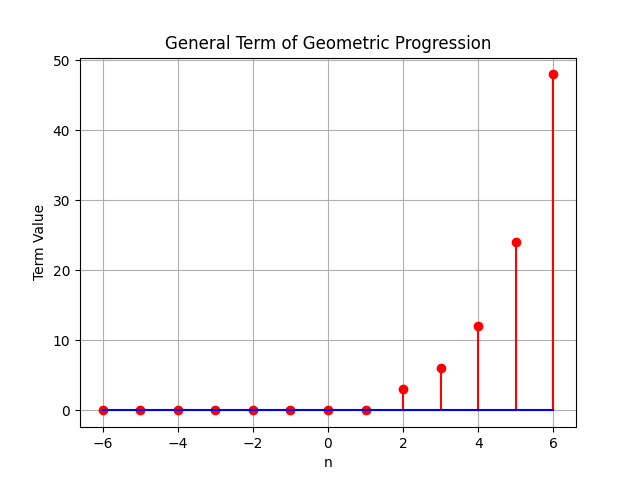
\includegraphics[width=1.0\linewidth]{Figure_1.png}
    \caption{Plot of the general term taken from Python}
    \label{fig:1}
\end{figure}\\
General term can also be written as\
\begin{align}
\boxed{x\brak{n} = 3\times2^{n}}
\end{align}\
Now on Z-Transforming, the expression which we get is\\
\begin{align}
X\brak{z} &= \sum_{-\infty}^{\infty}3\times2^{n}z^{-n}u(n)   \\
\implies X\brak{z} &= \sum_{-\infty}^{\infty}3\times\brak{\dfrac{2}{z}}^{n}u(n)
\end{align}
For the above series to converge, modulus of common ratio should be less than 1.
\begin{align}
\implies r &= \bigg|\dfrac{2}{z}\bigg|<1\\
        |z|&> 2
\end{align}
Therefore for all values given above, the above sequence shall converge.
On simplifying $X\brak{z}$, we get
\begin{align}
\boxed{X\brak{z}=\dfrac{6}{z-2}}\,\,\,  \forall \,\,\, |Z|>2 
\end{align}
\end{document}
